\chapter{Results}
test,test

\section{Virtual Prototyping of Cell Signals}

\subsection{Numerical investigation of immunomagnetic label density and size on quantitative magnetoresistive sensing of single cells and cell aggregates}
Signal Similarity For Cells With Varying Bead Coverages

Cross-Correlation between single dipole with sum magentic moment and surface covered with randomly distributed magnetic particles

simulation of cell rolling velocity and forces

%\\nas.ads.mwn.de\tuze\t03\AG-Hayden Studenten\00_Students\Johann Brenner\02_software\01-MRCyte\Magnetic cytometry signal modeling
\subsection{Single Cell Signal}

\subsection{Cell Aggregates}

\section{Reference Bead Surface Functionalization}

\subsection{Amine-Surface Biotinylation}
Streptavidin-Atto488 reference calibration
Anti-Biotin-PE working?
BNF-Dextran-Streptavidin unspecific binding?



\begin{figure}[htb!]
	\centering
	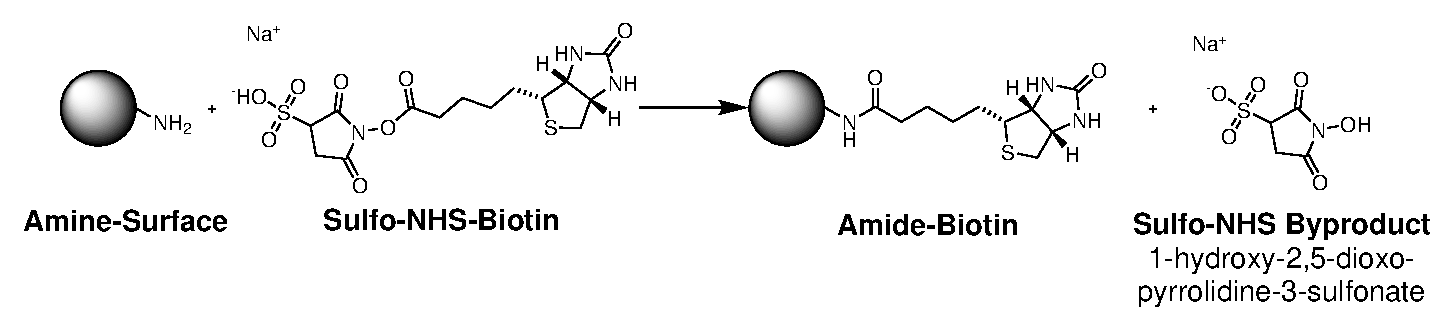
\includegraphics[width=\textwidth]{./Ressources/Chemistry/Sulfo-NHS.eps}
	\capption{Amine bead modification with Sulfo-NHS-Biotin}{An amine terminated bead is incubated with sulfo-NHS-Biotin to cover its surface by amide-Biotin. As byproduct the sulfo-NHS-ester 1-hydroxy-2,5-dioxopyrrolidine-3-sulfonate splits off. }
	\label{fig:Chem:NH2-NHS}
\end{figure}





\begin{figure}[htb!]
	\centering
	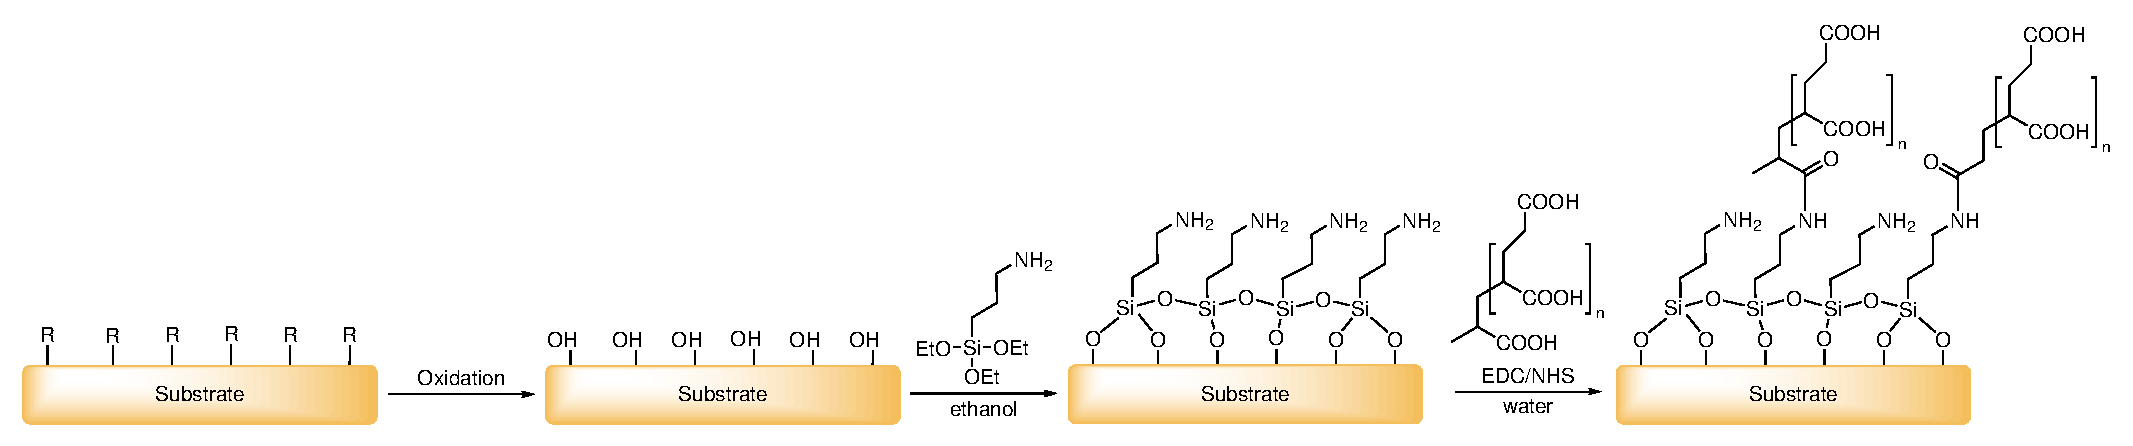
\includegraphics[width=1\linewidth]{Ressources/Chemistry/Substrate}
	\capption{General process chain of chemical surface modification}{Any substrate with various surface groups R (\textbf{a}) is oxidized to exhibit \gls{hydroxyl} groups.(\textbf{b}). Then a silane \gls{sam} is attached (\textbf{c}) and subsequently modified by carbodiimide chemistry with \gls{paa}. (\textbf{d})}
	\label{fig:chem:func:substrate}
\end{figure}



\subsubsection{Magnetic Polystyrene Bead}
\cleardoubleemptypage
\subsubsection{Non-Magnetic Polystyrene Bead}
\cleardoubleemptypage
\subsection{Carboxy-Surface Biotinylation}

\subsection{Surface Magnetization of Biofunctionalized Beads}

\todo{Results with ocean nanotec and bnf}

\section{Concentration Measurements in MRCyte}

\subsection{Count Stability}
Measurement over 1h
Measurement of Syringe Tubing Losses

\subsection{Calibration of Flow Field}

\subsection{Differential Counting Setup}

\subsubsection{Sensitivity Calibration}

\subsubsection{Concentration Measurements}
\cleardoubleemptypage

\section{Surface Modification and Biofunctionalization of the Sensor Chip Substrate}

\subsection{Physisorption}
Quantification in Plate Reader
Trial with Neutravidin + Sensor (Esthis Versuch)
\clearpage

\subsection{Covalent Attachment}
\clearpage

\subsubsection{Plasma-Based Approach}

\subsubsection{Water-Based Approach}
Sonicate in Acetone and Water 5'
1:1 \gls{hcl}:Methanol
\gls{h2so4}
Treat for 30 min in light boiling water